\section{}
\noindent 5. Considere el intervalo real $(-2,3] = \{x \in \mathbb{R} : -2 < x \leq 3\}.$ Para cada uno de los siguientes conjuntos universales encuentre $(2,3]^c$ y represéntelo en la recta real:\\
 
(a) $U = \mathbb{R};$
\begin{center}
$(-2,3]^c = \{x \in \mathbb{R} : x \leq -2$ y $x>3\}$\\
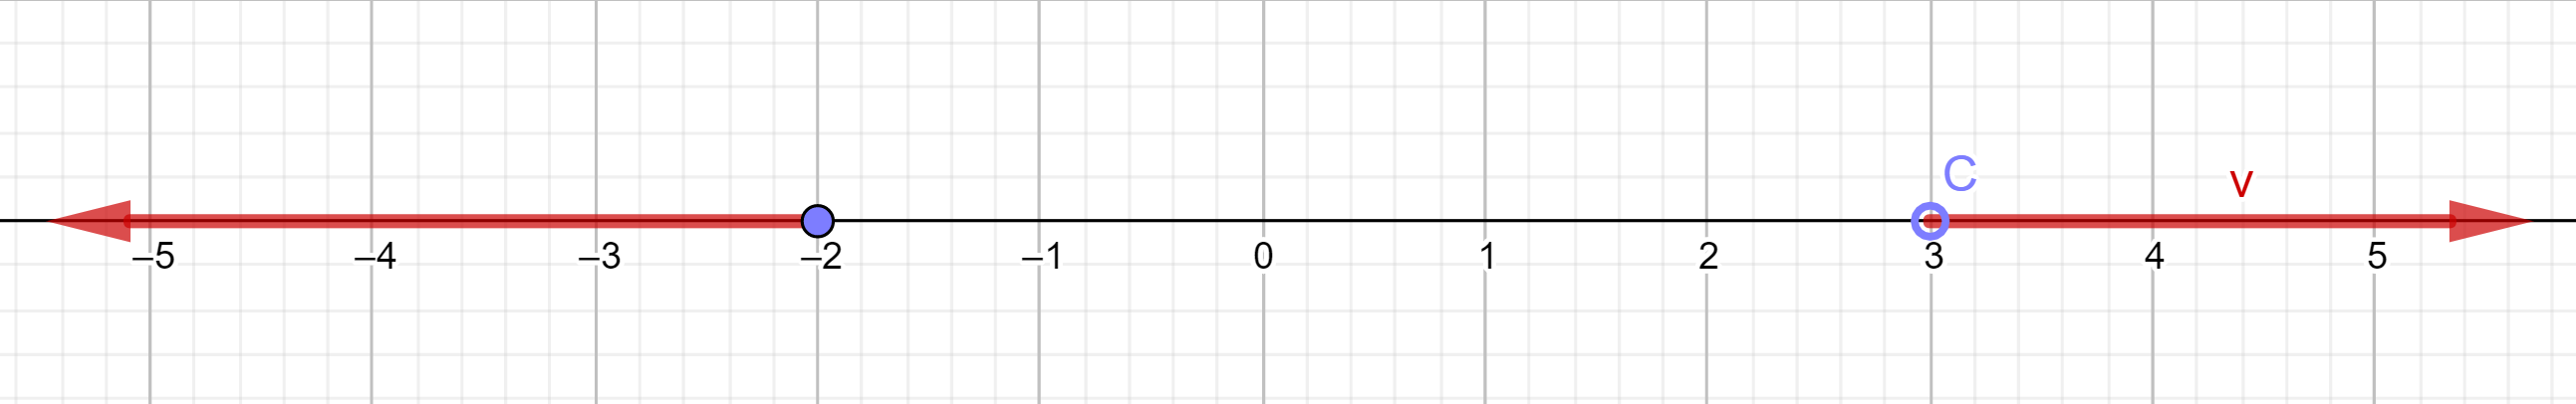
\includegraphics[scale=1]{img/problema_a.png} 
\end{center}
(b) $U = [-3,3];$

\begin{center}
$(-2,3]^c = \{x \in \mathbb{R} : -3 \leq x \leq -2\}$\\
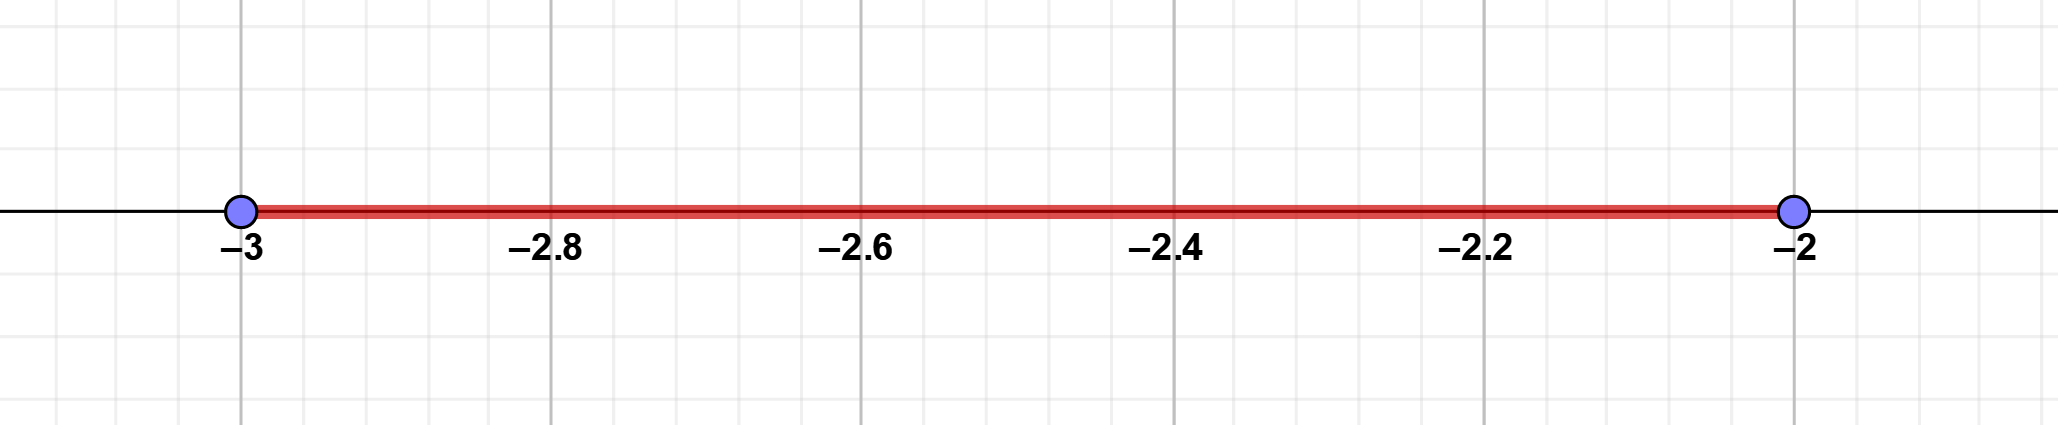
\includegraphics[width=12cm]{img/problema_b.png} 
\end{center}
(c) $U = (-\infty,5);$

\begin{center}
$(-2,3]^c = \{x \in \mathbb{R} : x \leq -2$ y $3 < x < 5\}$\\
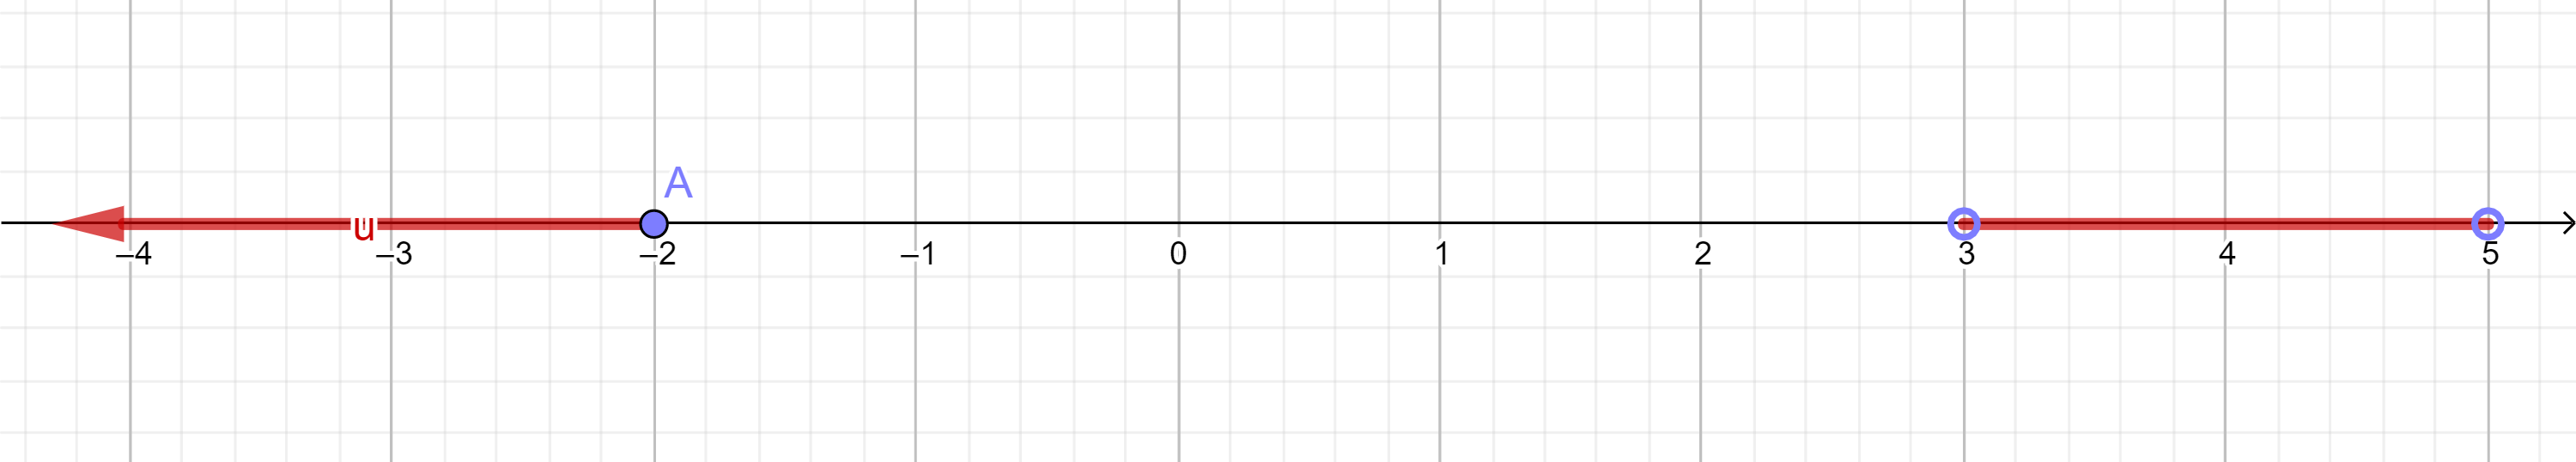
\includegraphics[width=12cm]{img/problema_c.png} 
\end{center}
(d) $U = [-2,10];$

\begin{center}
$(-2,3]^c = \{x \in \mathbb{R} : x = -2$ y $3 < x \leq 5\}$\\
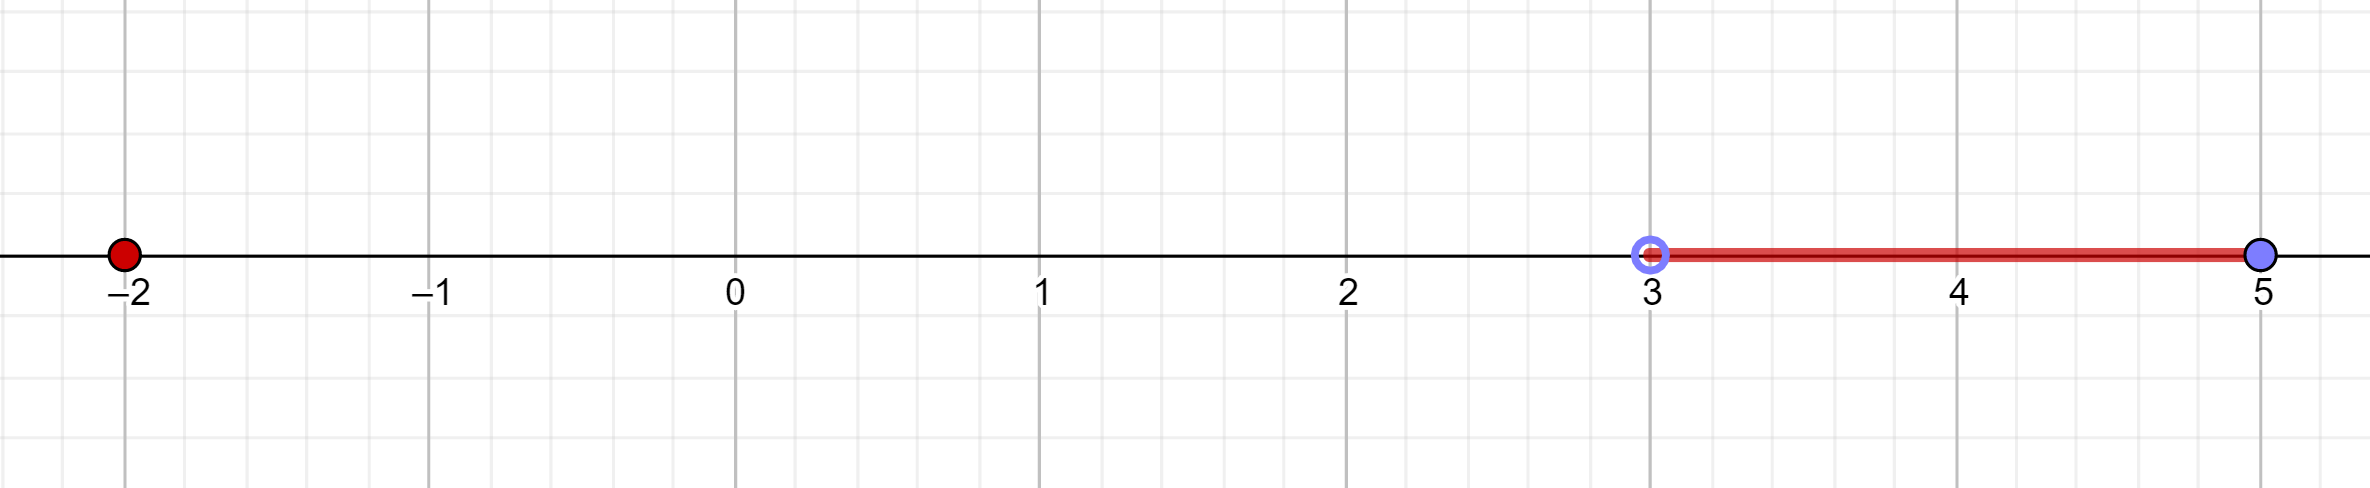
\includegraphics[width=12cm]{img/probema_d.png} 
\end{center}